\documentclass[11pt]{article}
\usepackage{longtable}
\usepackage{listings}
\usepackage{amsmath,amsfonts,amssymb,amsthm}
\usepackage[margin=1in]{geometry}
\usepackage[colorlinks]{hyperref}
\usepackage{algpseudocode}
\usepackage{algorithmicx}
\usepackage{listings}
\usepackage{multirow}
\usepackage{hyperref}
\usepackage{fancyhdr}
\usepackage{framed}
\usepackage{graphicx}
\usepackage{caption}
\usepackage{subcaption}
\usepackage{float}
\usepackage{enumerate}
\usepackage{tikz}
\usetikzlibrary{arrows}
\usetikzlibrary{shapes}

\newcommand{\C}{{\mathbb{C}}}
\newcommand{\F}{{\mathbb{F}}}
\newcommand{\R}{{\mathbb{R}}}
\newcommand{\Z}{{\mathbb{Z}}}
\newcommand{\e}[1]{\ensuremath{\times 10^{#1}}}

\newcommand{\ve}[1]{\boldsymbol{#1}}
\newcommand{\norm}[1]{\|{#1}\|}
\newcommand{\code}{\begingroup
	\catcode`_=12 \docode}
\newcommand{\docode}[2]{
	\begin{framed}
		\lstinputlisting[basicstyle=\ttfamily\scriptsize,language=#2,title=\underline{\texttt{#1}},tabsize=4,numbers=left]{#1}\end{framed}\endgroup}


\setlength\parindent{0pt}
\setlength{\parskip}{3mm plus3mm minus2mm}

\lstset{basicstyle=\ttfamily,showstringspaces=false}
\lstset{language=C++,
	basicstyle=\ttfamily,
	keywordstyle=\color{blue}\ttfamily,
	stringstyle=\color{red}\ttfamily,
	commentstyle=\color{gray}\ttfamily}

\begin{document}
	
	\thispagestyle{empty}
	%%%%%%%%%%%%%%%%%%%%%%%%%%%%%%%%%%%%%%%%%%%%%%%%%%%%%%%%%
	
	\title{Performance Evaluation of Docker}
	
	\author{Yuguang Zhang \\ University of Waterloo}
	
	\maketitle
	
	%%%%%%%%%%%%%%%%%%%%%%%%%%%%%%%%%%%%%%%%%%%%%%%%%%%%%%%%%
	
	\begin{abstract}
		Virtualization of operating systems provides a common way to deploy complex
		applications to a cloud environment. A new form of virtualization based on containers
		promises to offer better performance than traditional approaches with a virtual machine.
		This paper explores a method of running performance evaluation experiments using
		Docker and compares container based virtualization with native performance. Several
		benchmark tools are used to measure overhead in terms of processing, disk I/O,
		and memory performance. The results show that the performance of Docker containers is on par with native performance. In the Sysbench CPU benchmarks, the results on Docker and native differ by less than 1\%. In the memory and disk performance benchmarks, the memory and disk throughput in Docker are within 5\% of native performance.
	\end{abstract}
	
	\section{Introduction}
	Container-based virtualization is a lightweight alternative to hypervisor-based virtualization \cite{morabito}. Docker, a form of container-based virtualization, uses Linux kernel primitives to implement isolation of processes, network interfaces, and file systems. Creating a new container takes less than a second compared to minutes for spinning up a new virtual machine. This is because virtual machines run on virtualized hardware and virtual device drivers which present performance challenges due to the added layers between the physical hardware and the application. This paper explores Docker as an alternative to the reboot per job structure for running performance evaluation experiments in DataMill.
	
	DataMill is an infrastructure for rigorous and repeatable performance evaluation \cite{augusto}. DataMill executes the experiments on real hardware and incorporates the results from existing research on how to design experiments and evaluate hidden factors. The infrastructure automatically varies a selection of hardware and software factors, and therefore reduces the effort required by the user to set up and configure the experiment while simultaneously increasing the robustness and applicability of the experiments results to a wide range of factor levels \cite{augusto}. In order to execute experiments on real hardware and give users a clean workspace for experiments, DataMill currently makes a copy of the root filesystem to run benchmarks. DataMill workers consist of three partitions: boot, benchmark, and controller. The boot partition holds the kernel and grub. The controller partition is responsible for communication with the master node. The benchmark partition is where experiments are run. To run benchmarks, DataMill workers reboot into the benchmark partition. After running benchmarks, workers reboot to the controller partition.
	
	Docker is an alternative to the current dual boot structure while maintaining an isolated environment for each experiment. This paper explores the overhead of running benchmarks in Docker. The goal is to quantify the level of overhead introduced by Docker. The native performance is used as the reference for comparison. The main contributions of this paper are:
	\begin{itemize}
		\item An up-to-date comparison of container and native computing environments using recent software and generic workloads that measure CPU, memory, and disk I/O performance.
		\item A reliable way to execute benchmarks in a Docker container and compare the performance with the native performance as a baseline.
		\item A method for integrating Docker into the Datamill infrastructure for replicable performance evaluation experiments.
	\end{itemize}
	
	\section{Overview of Docker}
	
	Docker is a platform that allows developers to ``build, ship and run any app, anywhere". It is now the standard solution to software deployment, which is a costly and error prone process. One way to understand Docker is through a metaphor of shipping physical goods \cite{miell}. Before containers for shipping goods were invented, special handling was applied to different types of goods. Moreover, goods were shipped from sea to air, road to sea, sea to railroad, railroad to sea, and more combinations. For each of those cases, goods were handled differently. As a result, shipping was an expensive and difficult problem. To solve the complex problem of shipping goods cheaply to all locations, shipping containers were invented. These standardized containers had specific dimensions and weight. Ships and trucks were designed to carry, load, and unload these predictably shaped items. Different types of goods are packaged inside a container, and it doesn`t matter to the carrier what types of goods are in the container. Docker does the same thing for software rather than physical goods. Docker packages software dependencies and libraries in a standard format so that they are deployable anywhere.
	
	\subsection{How Docker is Used}
	Due to the lightweight nature of Docker containers, there are many versatile uses for them. These include prototyping software, modelling networks, and implementing a microservices architecture. Docker allows developers to experiment with new software setups without the hassle of starting a virtual machine. Since Docker provides a sandboxed environment, existing software installed on a development machine is not affected. Docker is also a portable way to package a software environment. A Docker image comes without any dependencies and runs as long as Docker is installed. Furthermore, Docker facilitates the development of a microservices architecture. One way to create a microservices architecture with Docker is to break down components into separate containers which are then composed to build a software stack \cite{miell}.
	
	Since a typical modern machine supports up to thousands of containers \cite{pahl}, Docker is a cheap and convenient way to model real world networks. Moreover, Docker simplifies debugging, as it allows developers to document exactly where a bug occurs and the steps to reproduce it. An added advantage of using Docker both in development and production is that the same container that runs on a developer’s laptop can run on a server. This simplifies remote debugging \cite{miell}.
	
	\subsection{Docker Architecture}
	Docker runs as multiple processes on a host machine. These processes include a client, a daemon, and a registry. The user interacts with the client to issue commands. The client sends HTTP requests to the Docker daemon, which runs as a service. The daemon in turn makes requests to other services to send and receive images. The daemon also manages the images and containers in addition to brokering interactions with registries. Docker Hub is an example of a public registry where users can share images with other users. In addition to public registries, many companies set up private registries for deploying and sharing images within the company. Docker registries are similar to source code repositories, and images can be pushed or pulled from these registries.
	
	Docker is built on LXC (LinuX Container) technology \cite{merkel} and uses kernel level primitives such as the copy-on-write filesystem, cgroups, and namespaces. Docker uses Linux namespaces to isolate the container from the host. This gives groups of processes a different view of the system. Docker uses several types of kernel namespaces, including:
	\begin{itemize}
		\item \texttt{pid} - Docker uses \texttt{pid} namespaces to separate processes within a container from processes outside it. With namespaces, processes within a namespace cannot see or influence processes outside of the namespace in other containers. Docker uses this feature to provide an isolated workspace within a container \cite{rosen}.
		\item \texttt{net} - The network namespace provides containers with its own network device and virtual IP address \cite{anderson}. For example, if multiple instances of Apache were running inside a container on port 80, Apache would not be exposed outside the container unless ports were mapped. Docker by default performs a network address translation to map ports from inside the container to the host.
		\item \texttt{mnt} - Docker allows host filesystems to be mounted in a container. This allows processes within a container to share files with the host and to have a different view of the filesystem from the host.
	\end{itemize}
	
	Docker uses control groups, often referred to as \texttt{cgroups}, to provide resource management and accounting. For instance, users can specify the amount of RAM or number of CPU cores for a container. \cite{anderson}. Docker provides granular control to physical resources, and users can add and drop capabilities.
	
	Docker relies on copy-on-write union file systems to provide a copy of the file system within containers. Docker uses Linux union file systems, which work by layering on top of existing file systems. Btrfs, device mapper, and AuFS are all examples of union file systems that support copy-on-write operations. Docker containers are built on a file system layer with libraries and binaries that fake an operating system. That base file system layer is referred to as an image in Docker terminology. Changes to the file system are added as layers and can be rolled back \cite{anderson}. The user may commit these changes and push them to a registry as an image.
	
	
	\subsection{How Docker Compares to VMs}
	Docker containers are quicker to spin up and deploy compared to virtual machines. Since Docker uses a layered filesystem, only the changes to the filesystem rather than an entire operating system will be shipped. As a result, Docker containers are lightweight to deploy and make changes to.
	
	Docker containers are lightweight and more scalable than virtual machines for running multiple instances on a single physical machine. In a scalability comparison done by Joy \cite{joy}, server instances were started up 22 times faster than virtual machines for a load balanced WordPress application. In this experiment, the AWS EC2 auto scaling feature is used. Auto scaling is triggered when the CPU utilization goes above 80\%. Jmeter is used to send concurrent requests to WordPress. Spinning up a new container to load balance the requests took only eight seconds compared to three minutes for a new virtual machine.
	
	Raho et al. conducted a performance analysis comparing KVM, Xen, and Docker on ARM based devices \cite{raho}. They found a negligible performance overhead for Docker and Xen privileged domains. On the UnixBench tests, hypervisors performed better than Docker on pipe-based context switches. This performance gain was attributed to caching in hypervisors. Xen and KVM also performed better than Docker IOzone benchmarks, except for the write operation. For small packets tested with Netperf, Xen performed the best. Docker had the best request/response performance.
	
	\section{Related Work}
	Morabit et al. \cite{morabito} compared hypervisor and container performance with running applications in a native environment. They used Y-cruncher, NBENCH, and Linpack to measure CPU performance under KVM, Docker, LXC, and OSV. In the Y-cruncher benchmark which measured multi-core efficiency, container based solutions performed better than KVM. In the NBENCH benchmarks, Docker and LXC performance was at the same level as native. The Linpack benchmark results showed that Docker and LXC had higher MegaFLOPS (floating point operations) than native. For disk I/O performance, sequential reads and writes of 25 GB was tested with Bonnie++. The results show that disk I/O efficiency is still a bottleneck with KVM, while the disk throughput for container based solutions were at the same level as native performance.
	
	Felter et al. \cite{felter} compare KVM and Docker performance with running applications in their native environment. In their benchmark, the Sysbench OLTP benchmark is compared against a single instance of MySQL. The benchmark compared MySQL throughput in terms of transactions per second on Docker with an AUFS volume, Docker with normal networking using NAT, and Docker using host networking and a mounted volume, native Linux, and KVM. The results showed that MySQL transactions under KVM qcow were about 30\% lower compared to native. Docker volumes have noticeably better performance than files stored in AUFS. They also found that NAT introduces overheads for workloads with high packet rates.
	
	Xavier et al. \cite{xavier} analyze MapReduce clusters and in HPC Environments comparing and contrasting the current container-based systems including Linux VServer, OpenVZ and Linux Containers (LXC). They evaluated the performance of MapReduce jobs on a cluster running different container systems. The results showed that all container-based systems offered a near-native performance. They also found that LXC was closest to native performance.
	
	\section{Methodology}
	The system parameters that affect the performance of an application running in Docker are the speed of the CPU, the speed of the memory, the speed of the hard drive, the Docker syscall overhead using Linux namespaces, and the Docker control group overhead. If the application communicates over a network, the speed of the network also affects performance. Since the syscall overhead and control group overhead are not factors that we can vary, we only consider the CPU speed, memory speed, and disk I/O throughput for our experiments \cite{bukh}. The workload parameters we considered that affect the performance are
	\begin{itemize}
		\item Prime number to calculate up to for the Sysbench CPU benchmark
		\item Different operations when running STREAM to test memory performance. These are vector ADD, TRIAD, SCALE, and COPY
		\item Small and large files for the file system benchmark
		\item Random and sequential operations for the file system benchmark
		\item Different operations for the file system benchmark (read and write)
	\end{itemize}
	We ran a number of benchmarking applications using Docker and used the native performance without Docker as the baseline. The benchmark tools measure CPU, memory, and disk I/O performance.
	
	\subsection{Software Environment}
	The host operating system used was Ubuntu 16.04 LTS with kernel 4.4.0-34-generic.
	The Docker image was based on the official Ubuntu 16.04 release image on Docker hub.
	Both the Docker image and native Ubuntu were configured using the default provided configuration files. Docker 1.12.0 was installed on the host OS running Ubuntu.
	
	\subsection{Hardware Environment}
	We used a Dell Precision 15 7000 laptop for our empirical experimentation, which had the following hardware:
	\begin{itemize}
		\item Intel Core i7-6820HQ
		\item 16 GB 2133 MHz DDR4 non-ECC SDRAM
		\item 256 GB M.2 PCIe NVMe High Performance Class 50 Solid State Drive
	\end{itemize}
	
	\section{Results}
	This section presents the results of the analysis. The benchmarks measure CPU, memory, disk I/O, and network I/O performance. Each individual measurement is repeated five 
	times and the diagrams show the average of the measurements. The error bars in the graphs indicate the
	standard error.
	
	\subsection{CPU Performance}
	The Sysbench CPU benchmark measures the execution time for a benchmark that finds prime numbers. The execution time is the end-to-end time from the start of the request to the end, which includes the overhead of shared memory access for the threads. The calculations are performed using 64-bit integers. Each thread executes the requests concurrently until the prime numbers up to a specified value are computed \cite{kopytov}. For this benchmark, we use two CPU workloads to represent high and low levels. For the lower CPU workload, we set the maximum prime number to 20000. For the higher CPU workload, we set the maximum prime number to 80000. 
	
	\lstset{caption=Sysbench CPU Benchmark Source Code, label=lst:Sysbenchcpu}
	\begin{lstlisting}[
	basicstyle=\small
	]
	int cpu_execute_request(sb_request_t *r, int thread_id)
	{
	unsigned long long c;
	unsigned long long l;
	double t;
	unsigned long long n=0;
	log_msg_t           msg;
	log_msg_oper_t      op_msg;
	
	(void)r; /* unused */
	
	/* Prepare log message */
	msg.type = LOG_MSG_TYPE_OPER;
	msg.data = &op_msg;
	
	/* So far we're using very simple test 
	prime number tests in 64bit */
	LOG_EVENT_START(msg, thread_id);
	
	for(c=3; c < max_prime; c++)  
	{
	t = sqrt((double)c);
	for(l = 2; l <= t; l++)
	if (c % l == 0)
	break;
	if (l > t )
	n++; 
	}
	
	LOG_EVENT_STOP(msg, thread_id);
	
	return 0;
	}
	\end{lstlisting}
	
	The Sysbench CPU benchmark source code is shown in Listing \ref{lst:Sysbenchcpu}. The event start time is logged before starting the prime calculation and the event end time is logged after the calculation. The \textit{cpu\_execute\_request} function is called 10000 times to calculate the average time it takes to compute the prime numbers. 
	
	
	\begin{figure}
		\centering
		{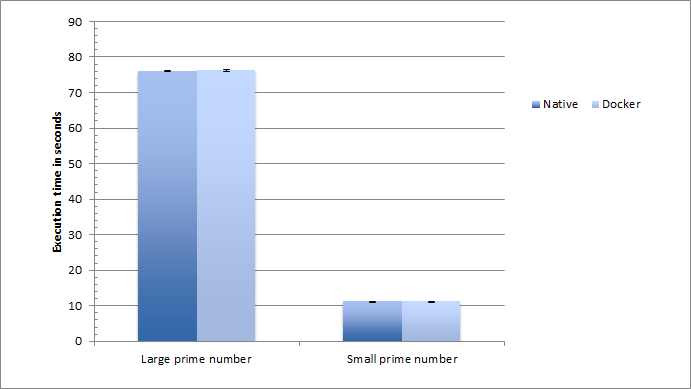
\includegraphics[width=150mm]{cpu.png}}
		\caption{ The value of Sysbench CPU benchmark results on over 10 runs}
		\label{fig:cpu}
	\end{figure}
	
	Fig. \ref{fig:cpu} shows the execution time of the Sysbench CPU benchmark where lower is better. The performance effect of running the benchmark in Docker is negligible, at about 0.1\%. For the benchmark with large prime numbers, the t-test statistic is -0.33021 and the p-value is 0.74972. For the benchmark with small prime numbers, the t-test statistic is 0.24674 and the p-value is 0.81491. Therefore, there is no significant difference in running the Sysbench CPU benchmark inside a Docker container and natively.  
	
	\subsection{Disk I/O Performance}
	Sysbench also has a set of file I/O benchmarks that characterize disk performance. There are three stages for a Sysbench I/O benchmark. In the \texttt{prepare} stage, Sysbench creates the files. The \texttt{run} stage is where the I/O operations for the benchmark are performed. Finally, there is a \texttt{cleanup} stage where files created for the benchmark are deleted. Sysbench supports many I/O operations, including:
	\begin{itemize}
		\item sequential write
		\item sequential read
		\item sequential rewrite
		\item random read
		\item random write
		\item combined random read/write
	\end{itemize}
	For the workloads, we have configured Sysbench to create a set of files with the total size of files to 5 GB. In order to clear the file system caches between each run, we unmount and format the file system. An example script for formatting a partition and mounting it in Docker to execute the random read benchmark is shown in Listing \ref{lst:Sysbenchio}. The accompanying Dockerfile in Listing \ref{lst:dockerfile} takes the \texttt{Sysbench-single.sh} script in the current directory and adds it to the working directory in the Docker image. Similarly, for measuring native I/O performance we unmount and remount a separate partition to clear the file system cache. 
	
	\lstset{caption=Sysbench File I/O Random Read Bash Script, label=lst:Sysbenchio}
	\begin{lstlisting}
	sudo mkfs.btrfs -f /dev/sdb1
	sudo mount /dev/sdb1 /mnt/benchmark/
	cat > Sysbench-single.sh <<EOF
	#!/bin/sh
	cd /benchmark
	Sysbench --test=fileio --file-total-size=5G prepare
	Sysbench --test=fileio --file-total-size=5G --file-test-mode=rndrd \
	run >> /results/Sysbench-file-randread.log
	Sysbench --test=fileio --file-total-size=5G cleanup
	EOF
	sudo docker build -t benchmark .
	sudo docker run -v /results:/results -v /mnt/benchmark:/benchmark \
	benchmark ./Sysbench-single.sh
	sudo docker rmi -f benchmark
	sudo umount /mnt/benchmark/
	\end{lstlisting}
	
	\lstset{caption=Dockerfile for Building Benchmark Image, label=lst:dockerfile}
	\begin{lstlisting}
	
	FROM yuguang/benchmark-64bit
	ADD . /scripts
	WORKDIR /scripts
	RUN chmod +x *.sh
	\end{lstlisting}
	
	
	\begin{figure}
		\centering
		{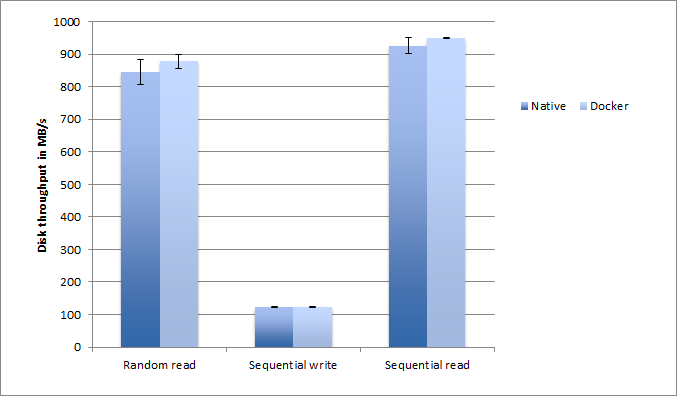
\includegraphics[width=150mm]{disk1}}
		\caption{ Disk Throughput achieved by running Sysbench.
			Results for sequential writes, sequential reads, and random reads are shown.
		}
		\label{fig:disk1}
	\end{figure}
	
	\begin{figure}
		\centering
		{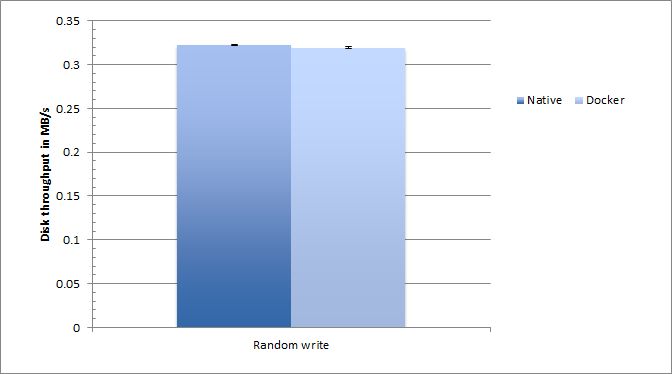
\includegraphics[width=150mm]{disk2}}
		\caption{ Disk Throughput achieved by running Sysbench.
			Results for random writes are shown.
		}
		\label{fig:disk2}
	\end{figure}
	
	The experiments were performed on an SSD. The results are summarized in Fig. \ref{fig:disk1} and Fig. \ref{fig:disk2}. For the random write benchmark, the p-value is 0.01720, which is greater than 0.05. Similarly, for the sequential write benchmark, the p-value is 0.74263. Therefore, the performance difference between Docker and native is not significant for random and sequential writes. For reads, the p-values are 0.28154 and 0.75729, respectively for random and sequential. This shows that the difference in read performance is also insignificant.  
	
	\subsection{Memory Performance}
	STREAM is a synthetic benchmark program that measures memory bandwith using simple vector kernels \cite{mccalpin}. It runs multiple repetitions of four different kernels: \textit{copy}, \textit{scale}, \textit{add}, and \textit{triad}. STREAM uses arrays that are at least four times larger than the sum of all the last level CPU caches in order to measure the main memory bandwith. The computed result is validated as an integrity test on the arrays. 
	
	\begin{figure}
		\centering
		{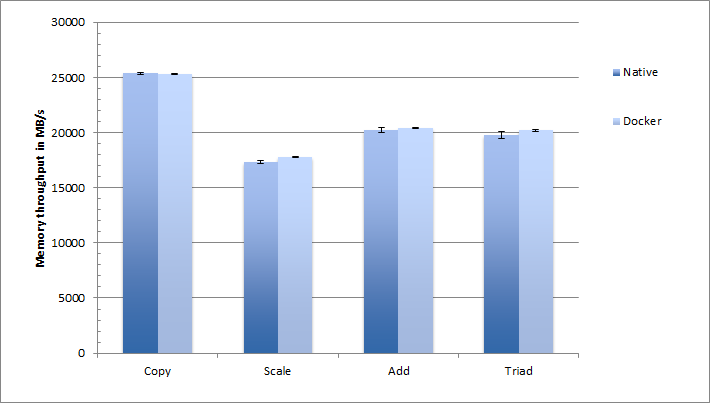
\includegraphics[width=150mm]{mem}}
		\caption{  Memory throughput is tested with STREAM. Measurements show
			that for all four operations the same level of performance is achieved for Docker and native. }
		\label{fig:mem}
	\end{figure}
	
	
	We ran the
	STREAM benchmark with an array size of 10 million elements, or
	a total memory requirement of 0.2 gigabytes. The particular CPU
	where we ran the benchmarks had 4 physical cores, each with a L2 cache size of 256 kilobytes and a L3 cache size of 1 megabyte. 
	Therefore, the CPU has a total L2 cache size of 1 MB and L3 cache size of 4 MB, which this test exceeded by
	two orders of magnitude. 
	
	The results from running STREAM 5 times are plotted in Fig. \ref{fig:mem} where throughput is in megabytes per second. 
	The test consisted of 10 repetitions of four of the kernels. The best results of the 10 trials are chosen to calculate the throughput \cite{mccalpin}. STREAM runs the code with many different offsets and chooses the best offset. The intent of STREAM is to find the memory bandwidth under optimal conditions \cite{mccalpin2}. 
	For all of the operations, the difference in throughput between running in a Docker container and natively is less than 3\%. For some operations, the best rates out of 10 were better higher in Docker than on native. This may be the result of better process isolation in a Docker container. 
	
	\section{Discussion}
	Execution time, memory throughput, and disk I/O throughput vary widely depending on the setup of the experiment. Nevertheless, if care is taken during the setup, the execution time, memory throughput, and disk I/O performance in a Docker container are similar to native performance. In the Sysbench CPU benchmarks, the results on Docker and native differed by less than 1\%. In the STREAM memory benchmarks, again the performance was the same with less than 3\% difference. Docker containers performed at about the same level in the Sysbench disk I/O benchmarks. Although the disk I/O benchmarks showed the greatest variation in the measurements, the performance difference was not significant. Overall, the differences in the execution time, memory throughput, and disk I/O throughput were not statistically significant based on the t-test statistics. 
	
	
	\subsection{Lessons Learned}
	In order to compare the performance of benchmarks running in Docker to their native performance, care must be taken for the experiment setup. For our initial experiment setup, we ran our benchmarks on the Datamill infrastructure with Gentoo workers. Datamill is an infrastructure for automating performance evaluation that runs packages across a group of distributed workers. Due to the lack of a Gentoo container, we built a Docker image for running the benchmarks with the necessary dependencies from Ubuntu. The results showed the memory and CPU intensive benchmarks performed better in the Docker container than on the native host. This was due to a mismatch of GCC versions in the Docker container and the Gentoo host. Gentoo used an older version of GCC. GCC on the Gentoo host were at version 4.9.3, compared to version 5.4.0 in the Docker container based on Ubuntu. As a result, the memory and CPU intensive benchmarks in the Docker container were more optimized than those run on the Gentoo host. 
	
	After switching to Ubuntu 16.04 for both the native baseline and the Docker container, the memory and  CPU intensive benchmarks had the same level of performance natively and in the container. However, the disk I/O benchmarks showed a performance gap with this round of experiments. After further investigation, we found that the mount options were different for the partitions in the Docker container and native baseline. We ran the native benchmarks in \texttt{/home}, while Docker stored container images in \texttt{/var}. \texttt{/home} was on a separate partition and had different mount options from the partition for \texttt{var}. 
	
	Another area of interesting performance variation between native and Docker container performance is with USB mounted partitions. With USB partitions, we found that the random write performance was much worse in Docker than on native. Random write throughput on native was 6 times the throughput in a Docker container. Also, the sequential write throughput on native was more than 10 times the throughput in a Docker container. Clearly, the kernel mount namespace or cgroups impose additional restrictions for USB partitions compared to hard drive partitions. These experiments were done on a removable USB drive where the file system was formatted and unmounted between test runs. The USB had a total capacity of 16 GB and a USB 3.0 interface. 
	
	\section{Conclusions and Future Work}
	
	Container based technologies are an interesting alternative to traditional virtual machines. Docker is a popular container technology that runs on Linux using kernel cgroups and namespaces. It is a lightweight alternative to hypervisor based technologies such as KVM. Docker facilitates the deployment of services and allows more software services to be deployed on a physical machine compared to traditional virtual machines. In this paper, the performance evaluation of Docker shows that benchmarks run on Docker have the same level of performance as on a native machine. 
	
	The results show that the performance of Docker containers is on par with native performance. In the Sysbench CPU benchmarks, the results on Docker and native were about the same. In the STREAM memory benchmarks, performance was at the same level again with no significant difference. In the disk I/O benchmarks, read and write operations in Docker performed at the same level as native. 
	
	One of the goals of this research paper was to Docker suitable for replicable performance evaluation experiments. In other words, the goal is to determine whether packaging benchmarks in a Docker container facilitate reproducing the same procedures, measuring systems, and operating conditions to obtain the measurements reported. There are two aspects to this. First, whether Docker aids in experimental setup portability. Second, whether Docker introduces a small enough overhead that measurements are similar to those made on a native machine. 
	
	Through experimenting with various setups, we have found that to reproduce native measurements, the GCC and libc versions must match those on the native machine. In addition, mounting a host volume in the Docker container yields the closest performance compared to native. However, care must still be taken to the filesystem and mount options to reproduce the same measurements. 
	
	In terms of experimental setup portability, Docker is an ideal solution. As long as the Docker daemon is installed on a host machine, it can run the software in the Docker container. This means that a Ubuntu OS in a container runs on a RedHat or CentOS machine with Docker installed. In addition, Docker packages software in a concise format, saving changes to a layered file system. This makes the artifacts used in experimental computer science portable and easily distributable. 
	
	\subsection{Integration with Datamill}
	
	Datamill is an infrastructure for automating performance evaluation that runs packages across a group of distributed workers. DataMill facilitates producing robust, reliable, and reproducible results by incorportating the latest research results on hidden factors and automating the variation of these factors \cite{augusto}. This section explores the possibility of integrating Docker into the Datamill infrastructure for replicable performance evaluation experiments. 
	
	Datamill workers have three standard partitions: boot, controller, and benchmark. The boot partition is for the kernel and initramfs, the controller partition holds a barebones Gentoo installation, and the controller partition is cloned to run benchmarks in the benchmark partition. As a result, the allocated disk space for the controller partition is minimal to give as much space to run experiments as possible on the benchmark partition. 
	
	Docker stores data such as images and containers in the user’s directory on disk. If the containerized experiments were run on the controller partition, the file system on the controller partition will inevitably run out of disk space. Therefore, the proposed way to run containerized experiments is by starting the Docker daemon with an argument to specify its directory. For example to run Docker from \texttt{/mnt/benchmark}, the command to start the Docker daemon is \texttt{docker -g /mnt/benchmark -d}. This will create a set of files and folders internal to Docker in \texttt{/mnt/benchmark}. After running an experiment files and folders in \texttt{/mnt/benchmark} are deleted, removing the containers and images. 
	
	\begin{thebibliography}{99}
		\bibitem{miell}
		Miell, Ian, and AidanHobson Sayers. \textit{Docker in Practice}. Manning Publications, New York, USA, 2015. Print.
		
		\bibitem{rosen}
		Rosen, Rami. \textit{Linux Kernel Networking}. Implementation and Theory. Springer Science and Business Media New York, New York, USA, 2013
		
		\bibitem{merkel}
		Merkel, Dirk. ``Docker: lightweight Linux containers for consistent development and deployment." Linux Journal 2014.239 (2014): 2.
		
		\bibitem{anderson}
		Anderson, Charles. ``Docker." IEEE Software 32.3 (2015).
		
		\bibitem{joy}
		Joy, Ann Mary. ``Performance comparison between Linux containers and virtual machines." Computer Engineering and Applications (ICACEA), 2015 International Conference on Advances in. IEEE, 2015.
		
		\bibitem{felter}
		Felter, Wes, et al. ``An updated performance comparison of virtual machines and Linux containers." Performance Analysis of Systems and Software (ISPASS), 2015 IEEE International Symposium On. IEEE, 2015.
		
		\bibitem{morabito}
		Morabito, Roberto, Jimmy Kjällman, and Miika Komu. ``Hypervisors vs. lightweight virtualization: a performance comparison." Cloud Engineering (IC2E), 2015 IEEE International Conference on. IEEE, 2015.
		
		\bibitem{mccalpin}
		McCalpin, John D.: ``STREAM: Sustainable Memory Bandwidth in
		High Performance Computers", a continually updated technical report
		(1991-2007), available at: ``http://www.cs.virginia.edu/stream/"
		
		\bibitem{mccalpin2}
		McCalpin, John D. ``Sustainable memory bandwidth in current high performance computers." Silicon Graphics Inc (1995).
		
		\bibitem{augusto}
		de Oliveira, Augusto Born, et al. ``Datamill: Rigorous performance evaluation made easy." Proceedings of the 4th ACM/SPEC International Conference on Performance Engineering. ACM, 2013.
		
		\bibitem{xavier}
		Xavier, Miguel Gomes, Marcelo Veiga Neves, and Cesar Augusto Fonticielha De Rose. ``A performance comparison of container-based virtualization systems for mapreduce clusters." 2014 22nd Euromicro International Conference on Parallel, Distributed, and Network-Based Processing. IEEE, 2014.
		
		\bibitem{kopytov}
		Kopytov, Alexey. ``SysBench manual." MySQL AB (2012).
		
		\bibitem{raho}
		Raho, Moritz, et al. ``KVM, Xen and Docker: A performance analysis for ARM based NFV and cloud computing." Information, Electronic and Electrical Engineering (AIEEE), 2015 IEEE 3rd Workshop on Advances in. IEEE, 2015.
		
		\bibitem{bukh}
		Bukh, Per Nikolaj D., and Raj Jain. ``The art of computer systems performance analysis, techniques for experimental design, measurement, simulation and modeling." (1992): 113-115.
		
		\bibitem{Sysbench}
		Kopytov, Alexey. ``SysBench: A System Performance Benchmark, 2004."
		
		\bibitem{estrada}
		Estrada, Zachary J., et al. ``A performance evaluation of sequence alignment software in virtualized environments." Cluster, Cloud and Grid Computing (CCGrid), 2014 14th IEEE/ACM International Symposium on. IEEE, 2014.
		
		\bibitem{pahl}
		Pahl, Claus. ``Containerisation and the PaaS cloud." IEEE Cloud Computing 2.3 (2015): 24-31.
		
	\end{thebibliography}
	
\end{document}